%---------------------------------------------------------------------
%
%                          Conclusiones y Trabajo futuro Ingl�s
%
%---------------------------------------------------------------------
\begin{otherlanguage}{english}
	
\setcounter{chapter}{7}
\chapter{Conclusions and Future Work}


%-------------------------------------------------------------------

This chapter will present the final conclusions of the project as well as possible improvements that could be made as future work if the project continues.

\section{Conclusions}

In today's society, communication is essential in the daily life of people, since it allows transmitting information and exchanging opinions and feelings with each other, which is essential as human beings. Today, society is not completely adapted to everyone's needs, since there are many people who have different disabilities: cognitive, physical, visual, auditory... Some of those with these disabilities can sometimes feel a little removed from the the rest for not having full access to information, such as the case of a person with a hearing impairment when listening to public address messages at a train station.\\

People with hearing disabilities have a lot of possibilities to communicate with others since the vast majority know how to read and write, but they also have a language of their own that is the Signs Language that allows them to express emotions and feelings when it comes to communicate. To help people with hearing disabilities, we saw it necessary to develop a tool that was capable of translating text into the SSL, since it could have many uses and facilitate the day-to-day life of people in this group. Some of these utilities could be learning the SSL, translating movie subtitles, or an informative text like airplane instructions to SSL...\\

The main goal of this project was to develop an application capable of translating any text in spanish into SSL in video, image or SSL text format, and Text2LSE has been developed for this.\\

Tex2LSE is currently capable of translating simple sentences that follow the structure TIME + SUBJECT + OBJECT + VERB, in addition to taking into account a large number of grammatical rules of the SSL, some of them being:



\begin{itemize}
	
	
	\item \textbf{Add verb tense: }Detect the verb tense of each phrase and add the corresponding sign either ``FUTURO'' or ``PASADO'' as can be seen in the Figure ~\ref {fig: AP_E15_cap8_in}.
	
	\begin{figure}[]
		\centering
		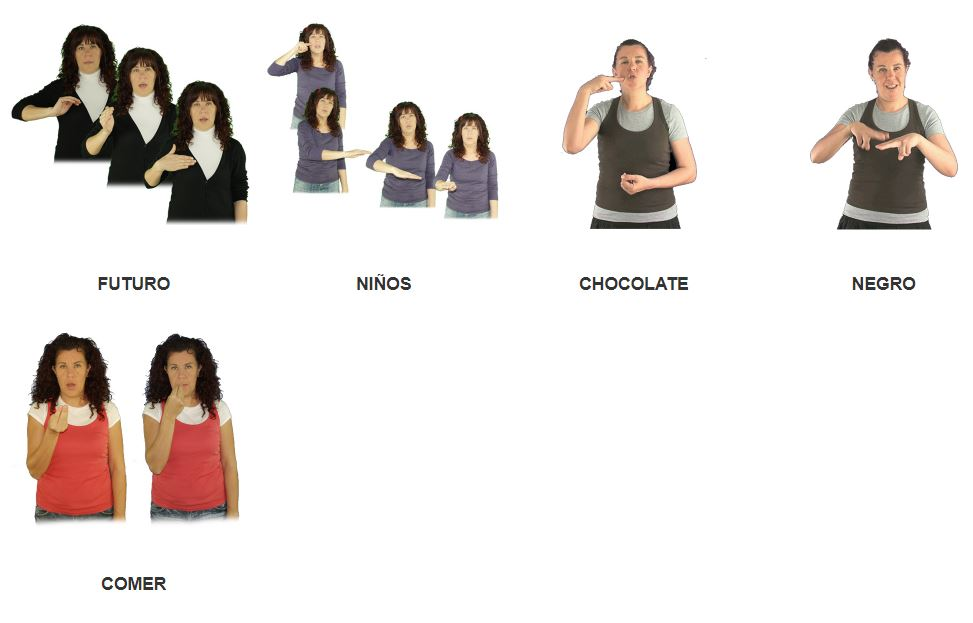
\includegraphics[width=1\textwidth]{Imagenes/Fuentes/Apendices/E15.jpg}
		\caption{Verbal tense and possessive sentence in SSL translated by Text2LSE }
		\label {fig: AP_E15_cap8_in}
	\end{figure}
	
	
	\item \textbf{Change possessive determinants:} The determinants that indicate possession are replaced by personal pronouns, as can also be seen in Figure ~\ref {fig: AP_E17_cap8_in}.
	
	\begin{figure}[]
		\centering
		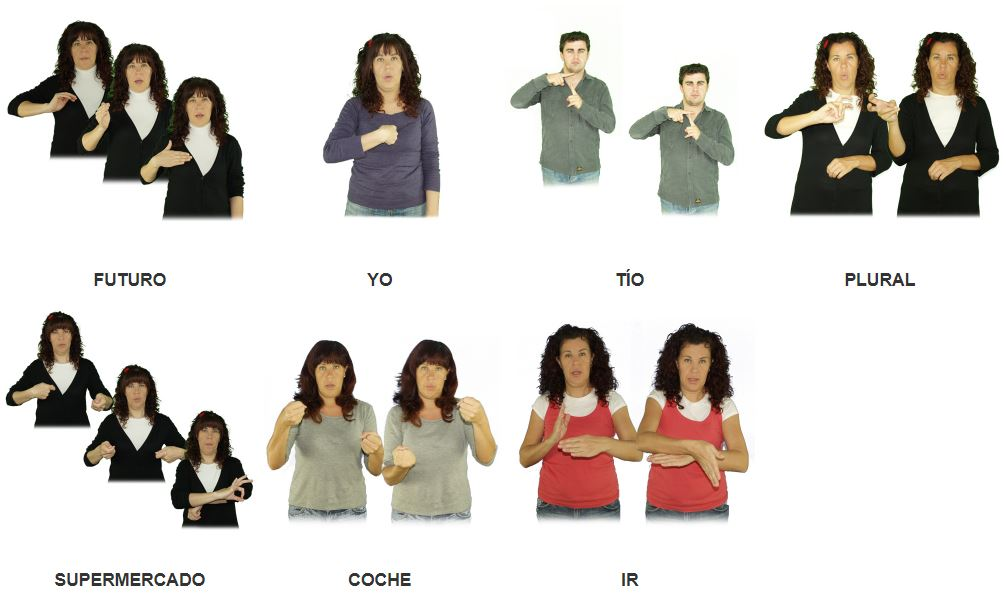
\includegraphics[width=1\textwidth]{Imagenes/Fuentes/Apendices/E17.jpg}
		\caption{Verbal tense and possessive sentence in SSL translated by Text2LSE }
		\label {fig: AP_E17_cap8_in}
	\end{figure}
	
	\item \textbf{Gender and number}: Detects the gender and number of each noun and indicates the sign of ``PLURAL'' in case of the number or ``MUJER'' in case of gender, as can be seen in the Figure  ~\ref {fig: AP_E16_cap8_in}.
	
	\begin{figure}[]
		\centering
		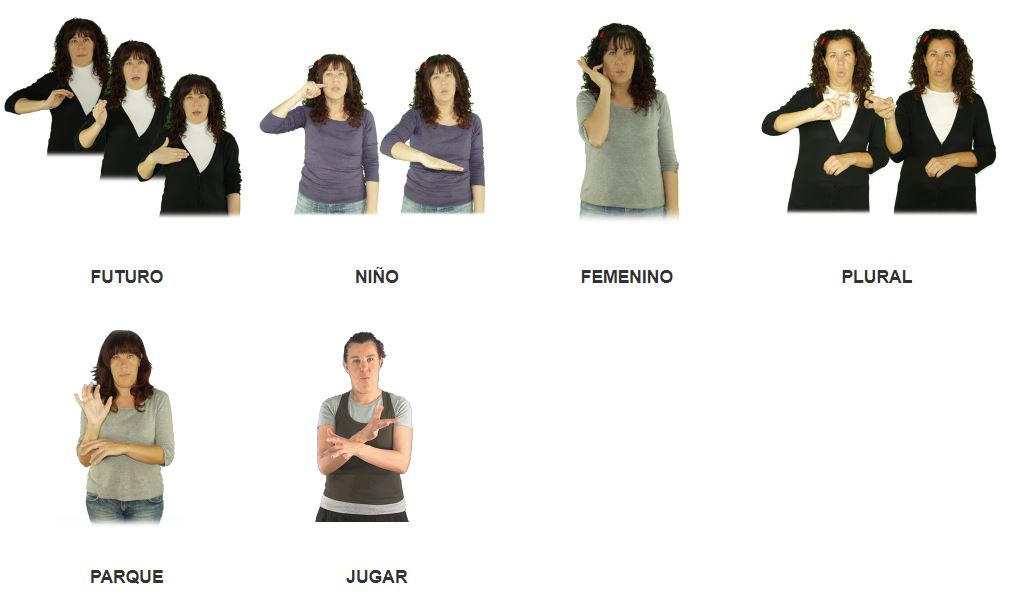
\includegraphics[width=1\textwidth]{Imagenes/Fuentes/Apendices/E16.jpg}
		\caption{Sentence with gender and number in SSL translated by Text2LSE}
		\label {fig: AP_E16_cap8_in}
	\end{figure}
	
	\item \textbf{Adjectives}: It detects all the adjectives of the sentence and passes them to singular masculine such as the Figure ~\ref {fig: AP_E2_cap8_in}.
	
	\begin{figure}[]
		\centering
		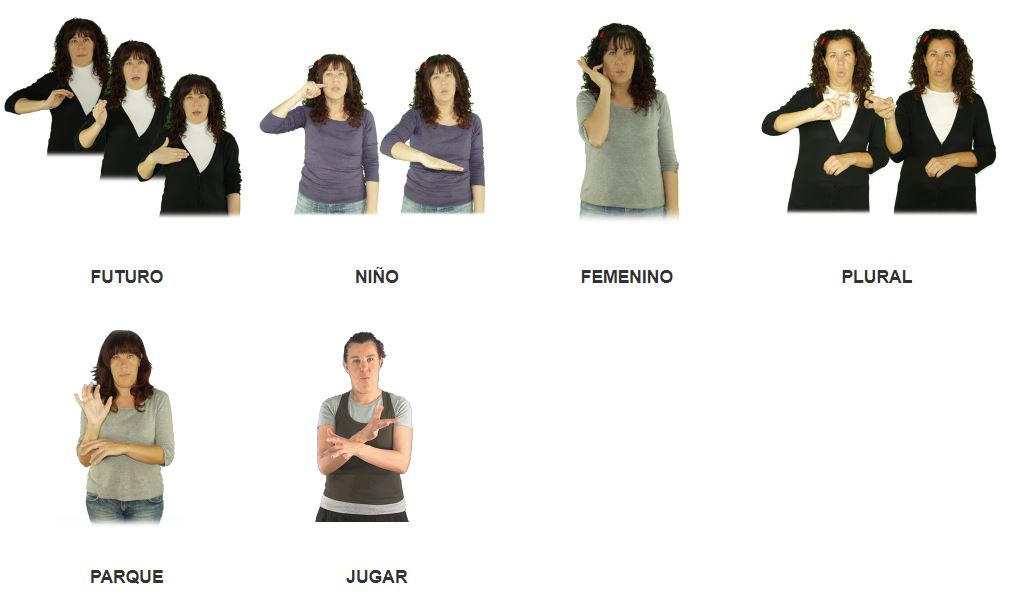
\includegraphics[width=1\textwidth]{Imagenes/Fuentes/Apendices/E16.jpg}
		\caption{Sentence with adjectives in SSL translated by Text2LSE}
		\label {fig: AP_E2_cap8_in}
	\end{figure}
	
	
\end{itemize}

Although there is a lot of work to be done, we would like to highlight that at the beginning of this project an analysis was made of different similar applications on the market, but we did not find any application that carried out text translations to SSL in real time, so we can affirm that still not being perfect the result, this work is a good base for the translation from natural language to Spanish Sign Language. \\

Another important aspect of the work we have developed has been creating a public API\footnote{\url{https://holstein.fdi.ucm.es/tfg-text2lse/}} with the developed web services, in such a way that it is easy to use in other projects.\\ 

Apart from translation, the purpose was also to create an application with an intuitive interface that is accessible to everyone from any device. It was intended to make an evaluation of the interface with real users but due to the Covid-19 it has not been possible to carry out such evaluation. Still, taking into account the opinions of the tutors in this regard and following their design advice, we believe that the interface is simple and intuitive and we meet the objective set.\\

The development of Text2LSE has allowed us to apply many knowledge acquired during the Computer Engineering Degree in a large project with a social utility, not only for the academic field. Some subjects that have been very important to carry out this project have been:

\begin{itemize}
	
	
	\item \textbf{Web applications: } It has helped us a lot when doing the Front-end since it gave us great knowledge about web development with HTML, CSS and Javascript that have been very useful for this project.
	
	\item \textbf{Programming Technology:} Thanks to this subject we learned to carry out a project in Java. Although the project is made in Python, the important thing about this course is that it gave us great knowledge when programming, so learning a new language like Python has not been so complicated.
	
	\item \textbf{Algorithmic Data Structure}: What has helped us the most in this subject has been knowing how to use recursion when programming, since it has been a fundamental pillar in the NLP.
	
	\item \textbf{Ethics, Legislation and Profession}: It is a subject that has taught us how to use the licenses with which to protect our work, as well as learning to use free software and to reference all the information used in the project well.
	
	
\end{itemize}

Also the project has allowed us to develop a lot of new knowledge that has not been taken in the degree, such as: Web Services, Proxies, NLP, Python...


\section{Future Work}
\label{cap8:sec:TrabajoFuturo_in}

With the aim of improving some functionalities of the Text2LSE application in order to obtain a more complete application and with greater coverage, we think that the following could be marked as future work:

\begin{itemize}
	
	
	\item \textbf{Proper names translation:} In the SSL, proper names can be translated using the sign of each letter to complete the name, or use a proper sign that defines the person. Currently the application detects the proper name but cannot find a translation, since there are no images or videos for that name, as can be seen in Figure  ~\ref {fig: AnaAlta_in}. The solution would be to use the sign of each letter of the proper name as can be seen in Figure ~\ref {fig: NombreBien_in}
	
	\begin{figure}[]
		\centering
		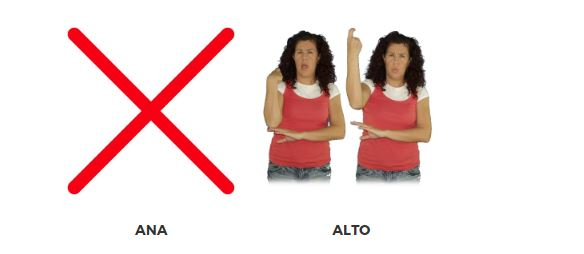
\includegraphics[width=1\textwidth]{Imagenes/Fuentes/Conclusiones/AnaAlta.jpg}
		\caption{Example of bad translation of a proper name made by Text2LSE }
		\label {fig: AnaAlta_in}
	\end{figure}
	
	
	\begin{figure}[]
		\centering
		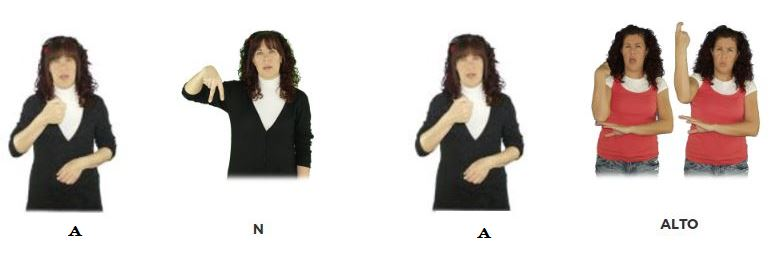
\includegraphics[width=1\textwidth]{Imagenes/Fuentes/Conclusiones/NombreBien.jpg}
		\caption{Example of a good translation of a proper name made by Text2LSE}
		\label {fig: NombreBien_in}
	\end{figure}
	
	
	\item \textbf{Improve Gender and Number:} As stated in section \ref{cap6:sec:An�lisis de los Resultados},An improvement would be to detect when to add the sign that indicates Feminine or the sign that indicates the Plural, since there are times when it is not necessary to add it, for example in the word ``rampas'' whose translation would be the sign \textit{``RAMPAS''} (Figure ~\ref {fig: rampas_in}). However, the application translates it as ``RAMPAS + FEMENINO + PLURAL'', as you can see in Figure ~\ref {fig: rampasMal_in}
	
	\begin{figure}[]
		\centering
		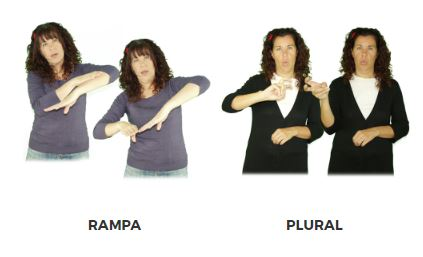
\includegraphics[width=0.6\textwidth]{Imagenes/Fuentes/Conclusiones/rampas.jpg}
		\caption{Correct translation of the word ``rampas'' by Text2LSE}
		\label {fig: rampas_in}
	\end{figure}
	
	\begin{figure}[]
		\centering
		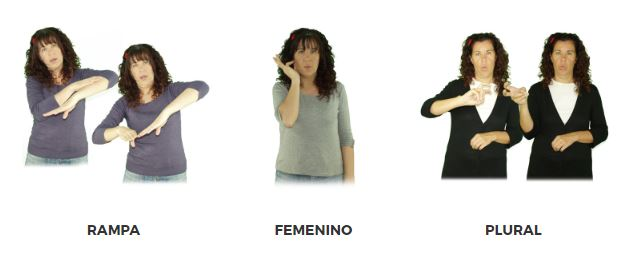
\includegraphics[width=1\textwidth]{Imagenes/Fuentes/Conclusiones/rampasMal.jpg}
		\caption{Incorrect translation of the word ``rampas'' by Text2LSE}
		\label {fig: rampasMal_in}
	\end{figure}
	
	\item \textbf{Add denial:} Currently the rule system does not contemplate the negation of sentences, so it would be a great advance to add a rule that allows a negative sentence to be translated well in SSL.
	
	\item \textbf{Recognition of compound times:} The application is currently not capable of recognizing compound tenses, such as ``han comido'' or ``estaban comiendo'', so it would be important to expand the NLP part of Text2LSE so that these types of verbs are translated from right way. In Figure ~\ref {fig: hanComidoPanMal_in} you can see that our application tries to translate the verb ``to have'' and finds no result. The correct option would be the one in Figure ~\ref {fig: hanComidoPanBien_in}
	
	\begin{figure}[]
		\centering
		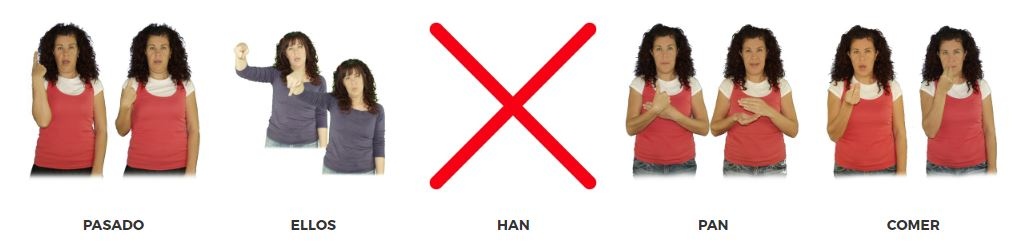
\includegraphics[width=1\textwidth]{Imagenes/Fuentes/Conclusiones/hanComidoPanMal.jpg}
		\caption{Example of bad translation of compound times made by Text2LSE}
		\label {fig: hanComidoPanMal_in}
	\end{figure}
	
	\begin{figure}[]
		\centering
		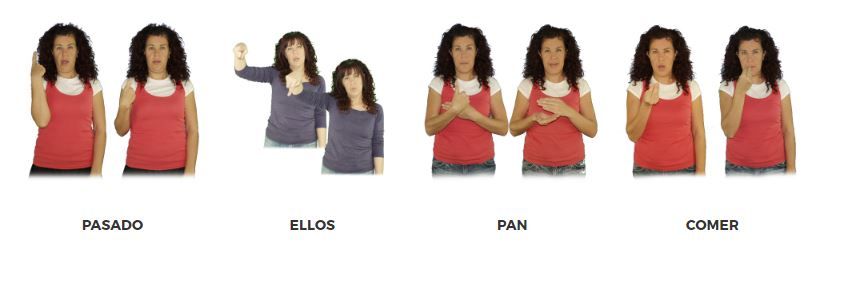
\includegraphics[width=1\textwidth]{Imagenes/Fuentes/Conclusiones/hanComidoPanBien.jpg}
		\caption{Example of good translation of compound times made by Text2LSE}
		\label {fig: hanComidoPanBien_in}
	\end{figure}
	
	\item \textbf{Treatment of phrases made:} Contemplate the identification of phrases made that have their own sign and does not require a word-by-word translation. For example, the phrase ``Secar el pelo'' is translated with a single sign, as can be seen in Figure ~\ref {fig: pelosecar_in}. However, our application performs the translation as if it were a normal sentence (See Figure ~\ref {fig: SecarPeloMAL_in})
	
	\begin{figure}[]
		\centering
		
\includegraphics[width=0.4\textwidth]{Imagenes/Fuentes/Conclusiones/pelosecar.jpg}
		\caption{Sign in SSL for the phrase ``Secar el pelo'' }
		\label {fig: pelosecar_in}
	\end{figure}
	
	\begin{figure}[]
		\centering
		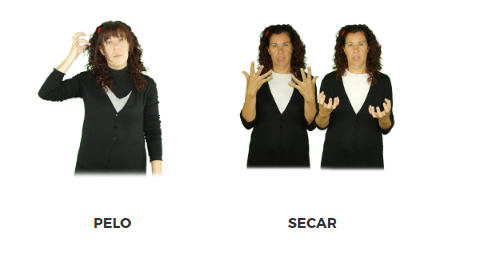
\includegraphics[width=1\textwidth]{Imagenes/Fuentes/Conclusiones/SecarPeloMAL.png}
		\caption{Sign in SSL for the phrase ``Secar el pelo'' made by Text2LSE}
		\label {fig: SecarPeloMAL_in}
	\end{figure}
	
	\item \textbf{Translation of compound sentences:} The current version of Text2LSE allows simple phrases to be translated, but does not translate compound phrases, such as ``Los ni�os fueron al parque para jugar con sus amigos'' In this sentence it can be seen that there are two simpler well distinguished sentences: ``Los ni�os fueron al parque'' and ``(Los ni�os) jugar con sus amigos''. A possible improvement would be to make a set of rules to translate these compound phrases.
	
	
	\item \textbf{Improvement in the System NLP:} The NLP used in the project has been through a system of rules using the Spacy tool. This system is not capable of translating phrases that are not contemplated in the previously programmed rules. An interesting and very important change would be to change the rule-based system to one based on machine learning, which is capable of learning by itself to translate any type of phrase based on training.
	
	
\end{itemize}


\end{otherlanguage}





%-------------------------------------------------------------------



